\documentclass{article}
\usepackage{graphicx} % Required for inserting images
\usepackage{hyperref}
\usepackage{fancyvrb}
\usepackage[backend=biber, style=apa]{biblatex}
\addbibresource{references.bib}
\usepackage{setspace} % Add this to your preamble


% Set smaller font size for all Verbatim environments
\fvset{
  fontsize=\small
}

\title{Methodology for Predictive calculator}
\author{Anton Mukin}
\date{June 2025}

\setlength{\parindent}{0pt}


\begin{document}

\maketitle

\subsection{Brief Summary of the Project}
This Matura project investigates and evaluates the arithmetic capabilities 
of different neural networks. 

The project began with a literature review to 
generate a hypothesis regarding the weaknesses of neural networks in 
performing simple arithmetic. This literature review was submitted as the 
Zwischenprodukt, alongside a proof-of-concept notebook featuring a 
comparison of Feed-forward Neural Networks (FNNs) of different sizes.

The next step was to build a Recurrent Neural Network (RNN) and similar 
attention-based RNNs to investigate their arithmetic capabilities and 
compare them to those of the FNN using a benchmark.

The benchmark's baseline was defined to be the performance of a basic FNN's 
performance on different, but roughly still similar arithmetic tasks.

Afterwards, the same was done for the transformer type of neural network 
model. Here, their exact functionality was thuroughly investigated, because 
of their unique architectures.

Lastly a simillar workflow was repeated for some bigger, pre-trained models. 

And finally all the findings were collected and evaluated as a whole.


\subsection{Introduction to this document}
The goal of this document is assisting reproducability and showing how the 
findings discussed in the other document have been obtained.

All of the code written for this project is available in the github 
reporsitory: 

\url{https://github.com/AntonStantan/matura}

In this project all of the code is written in Python-notebooks (Jupyter Lab).
The preffered library used was \href{https://www.tensorflow.org/guide/keras}
{tensorflow keras}. 

Most of the models were trained locally on a Nvidia GPU device: \textit{Nvidia 
Jetson Orin Nano Super Developer Kit}

\begin{figure}[htbp]
    \centering
    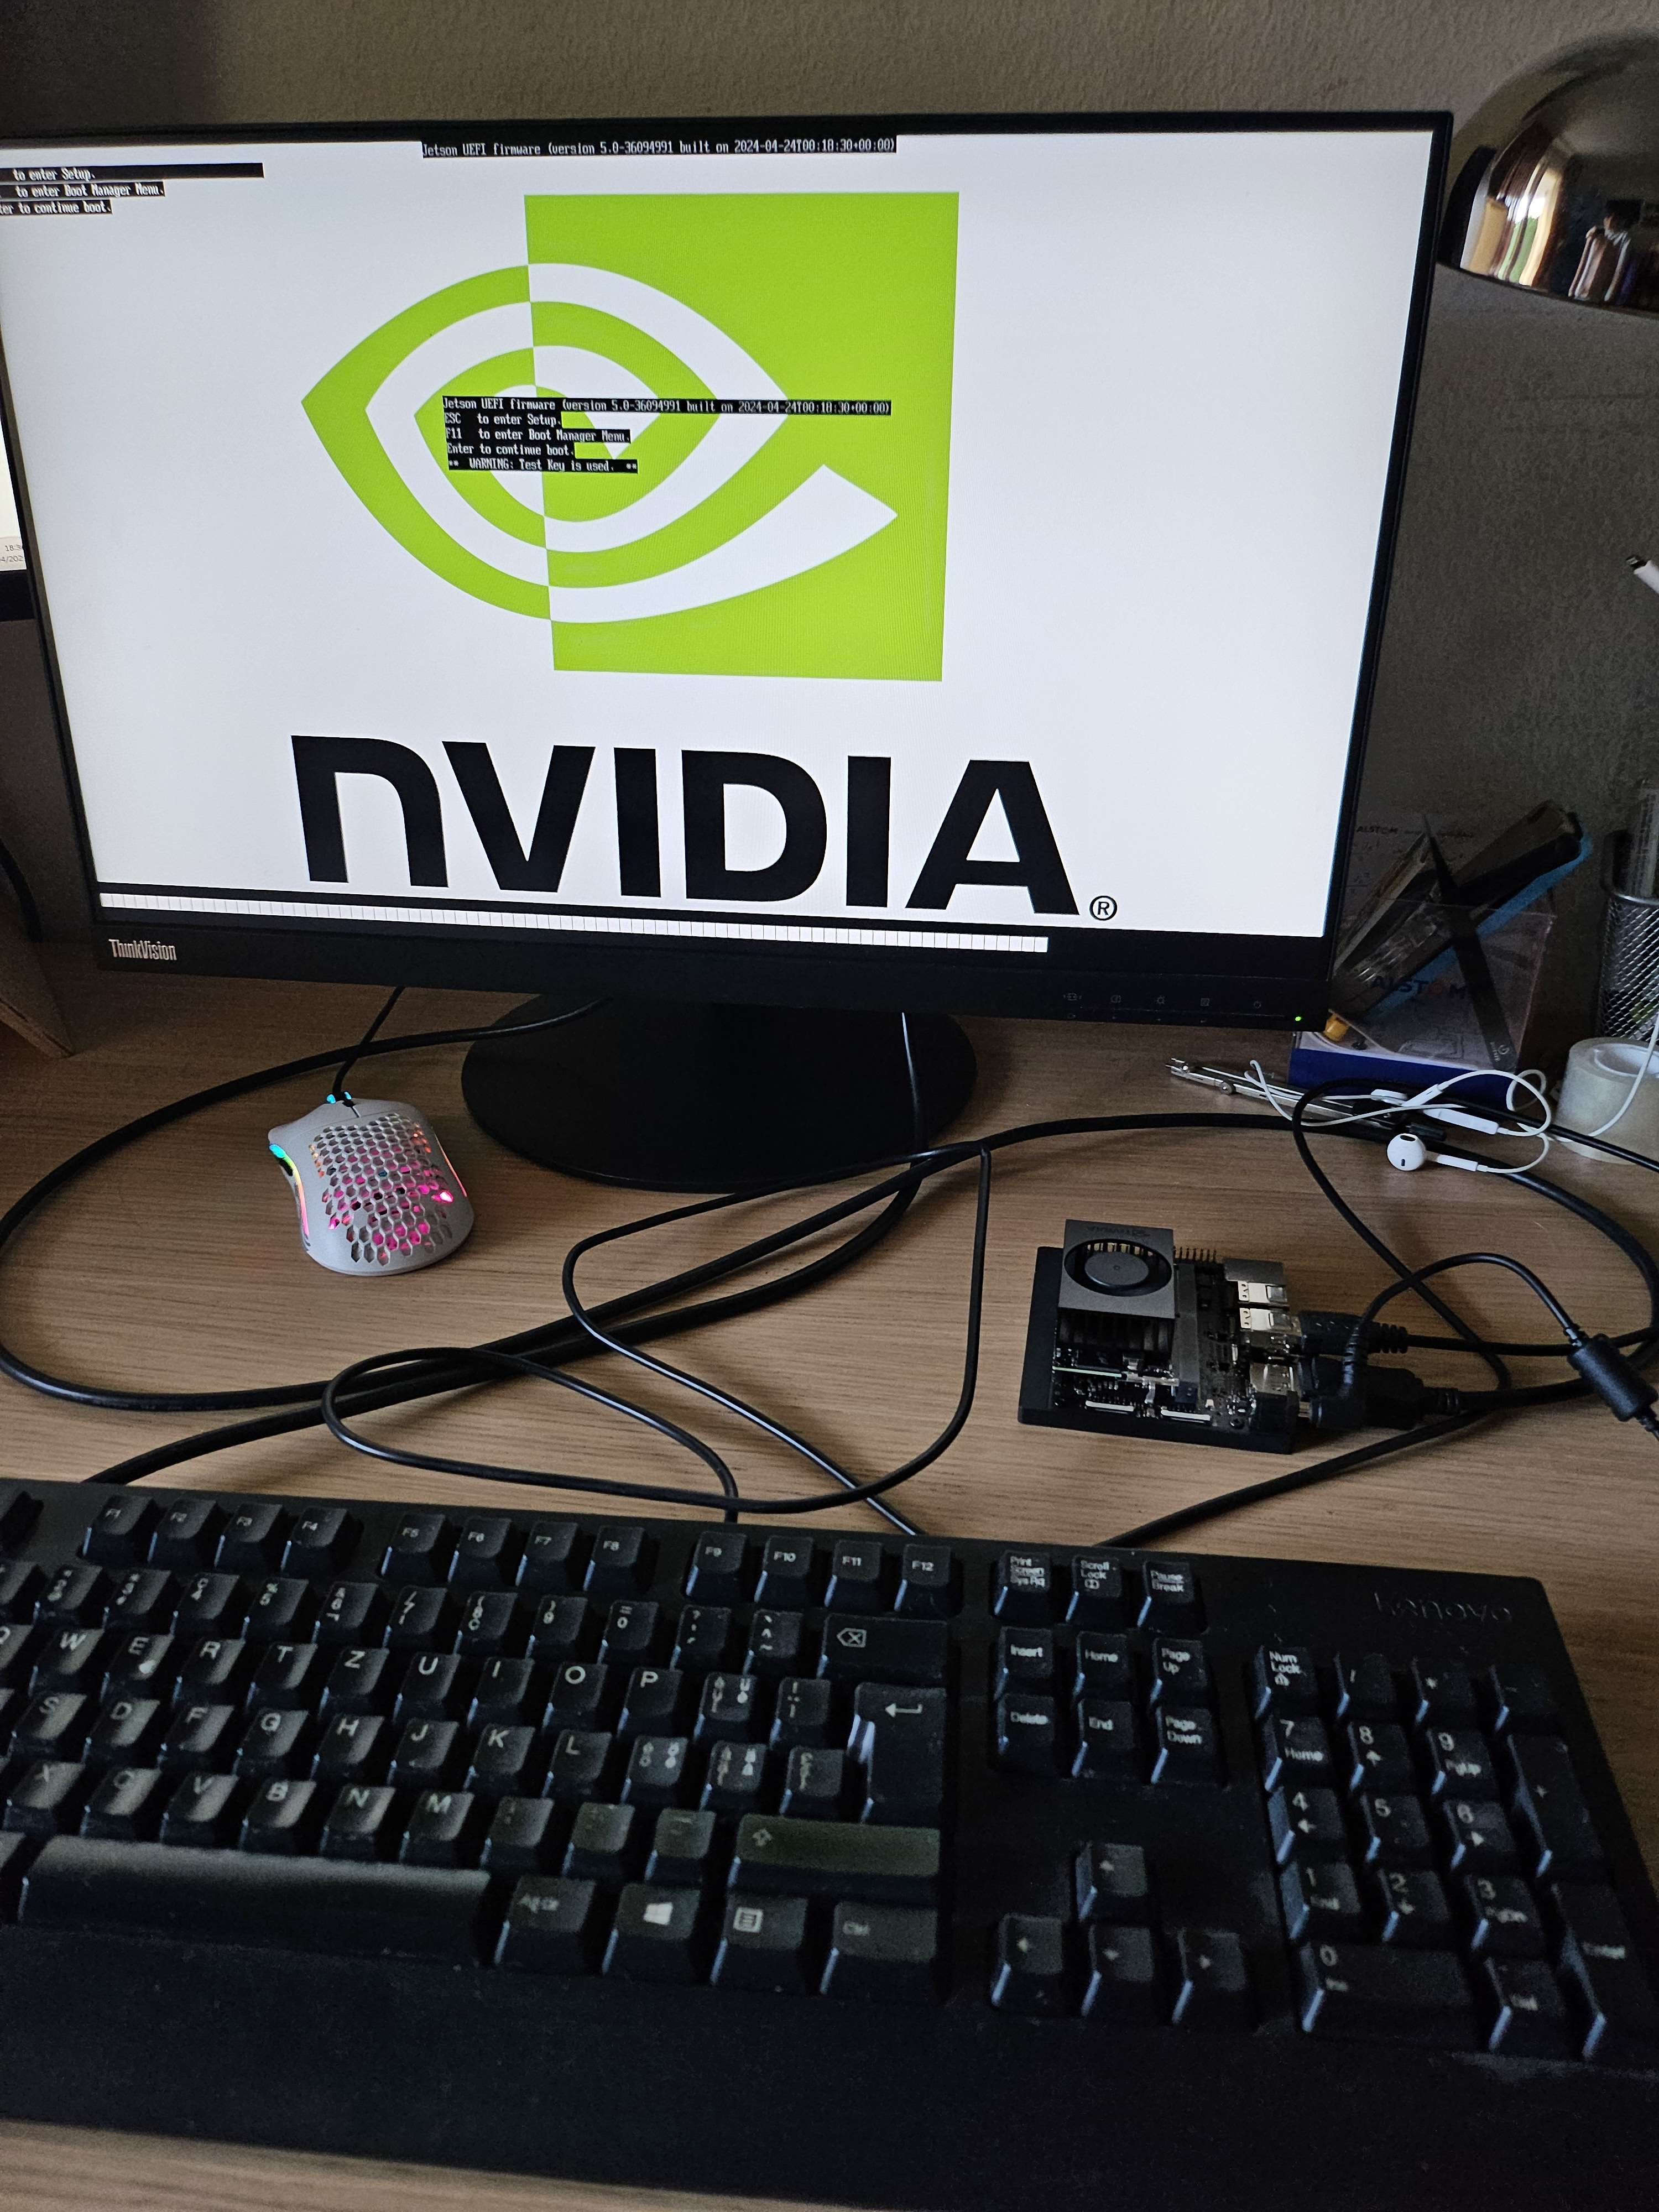
\includegraphics[width=0.5\paperwidth]{images/JetsonBoot.jpg}
    \caption{You can see the aformentioned Nvidia Jetson device booting up.}
    \label{fig:JetsonBoot}
\end{figure}

\newpage
\tableofcontents
\newpage

\section{Feed-forward Neural Networks (FNN)}
For details on how a FNN works please refer to the section two in \href{https://github.com/AntonStantan/matura/blob/main/zwischenProdukt/LiteraturstudieAnton.pdf}
{the literature study}.

This section refers to the \href{https://github.com/AntonStantan/matura/tree/main/FNN}
{/FNN directory} in the github reporsitory.

There are two notebooks here: \href{https://github.com/AntonStantan/matura/blob/main/FNN/FNN1.ipynb}
{FNN1} and \href{https://github.com/AntonStantan/matura/blob/main/FNN/FNN2.ipynb}
{FNN2}.

\subsection{Train and Test data}
Defining the train data; The decision was made to only use subtraction and 
addition. The arithmetic expressions were defined to consist of two 
operators (+ or -) and three integers $[-5, 5]$

The reason for these definitions are: + and - are the 2 simplest operators. 
And the decision to introduce the model to 3 numbers, in place of the more 
commonly used 2, was made in hopes of simplifying the transition to more 
numbers later on.

e.g., the first three entries are: 
\[
1 - -2 + 3 \qquad -2 + -3 - -5 \qquad 3 - 1 - 0
\]
{\small In total there are 1907 expressions like this in the train data.}
\\[2em]
The test data is also defined in a slightly unconventional manner. It is 
split up into three categories.
\begin{itemize}
    \item Inside of the number range: Expressions just like in the train 
data but not inside of train data. 
    \item Outside of the number range: The same expressions, but with 
numbers in the ranges $[-8, -5]$ and $[5, 8]$ e.g.,
\[
-6 + 6 + 8 \qquad -7 + 6 + 7 \qquad 5 - -6 - 6
\]
    \item Longer expressions: Expressions of different lengths. 
Specifically, there are between 2 and 8 numbers inside of the $[-5, 5]$ 
range. e.g.,
\[
-5 + 1 \qquad 3 + -1 + 4 + -2 + -4 \qquad -2 + 1 + 5 + -5 - -2 + -1 - 2 - 5
\]
\end{itemize}

\subsection{Tokenizer}

Because only tensors with floats can be passed into a model, the train 
and test data is always processed before entering a neural network in a 
tokenizer.

Traditionally a tokenizer assigns each character prevelant in data a number, 
but because we are working with numbers this isn't the case for us. Only the 
characters $+$ and $-$ need to be assigned a number.

For this project: the decision was made to work with: $1.0$ replacing $+$ and 
$0.0$ replacing $-$.
\\[2em]

Padding is also added, because a network that was trained on expressions with 
up to 3 numbers won't be able to pass higher dimensional vectors.

To differenciate it from all the other integers, a padding value of $0.5$ was 
defined.
\\[2em]
With that being said, an expression, after being passed throught the tokenizer 
would look something like this: 
$$
[1.\qquad 0.\qquad -2.\qquad 1.\qquad 3\quad 0.5\quad 0.5\quad 0.5\quad 0.5\quad 0.5\quad 0.5\quad 0.5\quad 0.5\quad 0.5\quad 0.5]
$$
\subsection{Training a Neural Network Using Tensorflow}
This subsection will show how the models used in this project were first 
defined and then trained with tensorflow on the example of a simple FNN.
\\[2em]
To start of we will import the necessary libraries.
\begin{Verbatim}
import tensorflow as tf
from tensorflow import keras
from tensorflow.keras.layers import Dense, Layer, Dropout
from tensorflow.keras import layers, Sequential
from tensorflow.keras.layers import PReLU
\end{Verbatim}

And then we have to make a dataset out of the train and validation data 
discussed in the previous subsection. Let's use batches of 32.
Validation data is like the In-Range-test-data, except there aren't as many
expressions.
\begin{Verbatim}
batch_size = 32
train_dataset = tf.data.Dataset.from_tensor_slices((x_train, y_train))
.shuffle(len(x_train)).batch(batch_size)
val_dataset = tf.data.Dataset.from_tensor_slices((x_val, y_val))
.batch(batch_size)
\end{Verbatim}

We can now define the model using tf.keras.Sequential. The model's 
architecture is clearly visible. In this example the model has two dense 
layers with 64 neurons each.

The activation function used is PReLU, as this is the one, which was the  
most promising in \cite{trask2018neuralarithmeticlogicunits}. 

Drop-out is included to prevent overfitting. In most models used in this 
project it wasn't necessary.

As you can see, the input-shape has to be defined, when defining the model.

Additionally, please notice how the output layer only consists of a single 
neuron with a linear activation function. This means the model we just 
created is a regression model. This is similar to not having a decoder.
\begin{Verbatim}
input_shape = (15,)
model = Sequential([
    keras.Input(shape = input_shape),     #input

    Dense(64),                            #first dense layer
    PReLU(),                              #PReLU activation function
    Dropout(0.1),                         #dropout layer

    Dense(64),                            #second dense layer
    PReLU(),                                
    Dropout(0.1),                           

    Dense(1, activation='linear')         #output layer
])
\end{Verbatim}

The next step is to compile the model, by choosing an optimizer and loss 
calculation e.g., in our case Mean Squared Error (MSE)
\begin{Verbatim}
model.compile(optimizer="adam", loss="mse")
\end{Verbatim}

The last step remaining is to fit the model on some data. We will be 
fitting our model on the previously defined train and validation data. 
The training process will take 200 epochs to complete or it might be aborted
preemtively if the model starts to overfit and early\_stopping is triggered.

\begin{Verbatim}
model.fit(
    train_dataset,
    validation_data=val_dataset,
    epochs=200,
    callbacks=[early_stopping],
    verbose=1
)
\end{Verbatim}

\subsection{FNN1 and FNN2 Notebooks}
In this project two notebooks with FNNs have been created. FNN1 and FNN2. 
In FNN1 a simple FNN was created, it's performance was evaluated and FNNs 
of different sizes have been compared against eachother in a heatmap. It is 
noteworthy, that the models here have been used with a bootstrap, meaning 
multiple models with the same sizes were trained and then used to give one 
combined prediction. This was done to reduce noise. In later notebooks this 
will not be the case, as this makes it more difficult to accurately evaluate 
a model.
\\[2em]
FNN2 includes a model with hyperparameters (in this case the number of 
neurons, the number of layers and whether or not to use dropout) chosen by 
the keras-tuner. This is simply put an automatization: It picks out models 
with different hyperparameters, trains them and compares their performance 
on validation data. The model with the best-performing hyperparameters will 
be chosen as the best model.

The model in FNN2 is evaluated inside of that notebook and it's benchmark 
is calculated.

\subsection{The Benchmark}
To calculate the benchmark a model is evaluated on 4 categories: The test 
data inside of the number range, outside of the number range, longer 
expressions and a relative MSE of the test data with numbers outside of the 
range.
Refer to the code below:
\begin{Verbatim}
benchmark = 0
benchmark += baseline_deviation / (meanDiff_InRange**2) / 4
benchmark += baseline_out_deviation / (meanDiff_OutRange**2) / 4
benchmark += baseline_long_deviation / (meanDiff_LongRange**2) / 4
benchmark += baseline_relError / (meanDiff_OutRelRange**2) / 4
print(f"Benchmark: {benchmark}")
\end{Verbatim}

The usage of a relative error punishes mistakes on "simpler" expressions and 
is less harsh on more "difficult". Expressions whose absolute result is 
small, are easier for a neural network to solve, while a larger absolute 
result is more difficult to calculate.

For the same reason two more adjustments have been made:
Not all expressions outside the number range, and not all longer expressions 
were used. 

For longer expressions only expressions with 4 numbers were used.

For expressions with numbers outside of the range, the expression was only 
used if the absolute values of all three numbers added up to 22.

These subsets were chosen because of their reasonable MSE of around 10 each.

This, aswell as the inlusion of the relative MSE is done in hopes of 
bringing the benchmarks of different models closer together and to increase 
the linearity between them. This makes the benchmark more comfortable to 
work with.

The baseline values are defined to be of a FNN model with 30 neurons and two 
dense layers. It is trained over the period of 200 epochs with 
early\_stopping enabled.

As clearly observable in the code for calculating the benchmark, using this 
formula defines a model with the same performance as the baseline model to 
have a benchmark of 1. Models performing worse or better on the test data 
yield scores below or above 1, respectively.


\subsection{Drop-Out}
When introducing a Drop-Out with an industry standard value of 0.3, contrary 
to the expectation of reducing over-fitting, which in some way is present 
(according to literature discussed in the literature study), as the models 
aren't able to generalize beyond the training range, this has a negative 
effect on the model. The MSEs of models with Drop-out are higher then, the 
ones of the previous models without drop-out. 

This is because drop out effectively decreases the computing cpacity of a 
model during training (when predicting this is no longer the case), by 
deactivating a percentage of randomly chosen neurons in each layer.
% https://github.com/AntonStantan/matura/blob/main/FNN_Heatmaps/DropOutComparison.png
%THIS SHOULD GO INTO FINDINGS

\section{Recurrent Neural Network (RNN)}

\subsection{RNN0 and RNN2}
The RNN0 notebook includes a model built with the aformentioned architecture.

A RNN model consisting of 2 dense layers with 50 neurons each:

\begin{Verbatim}
model = keras.Sequential([
    keras.Input(shape=(input_shape, 1)),
    keras.layers.SimpleRNN(50, return_sequences=True),
    keras.layers.PReLU(),
    keras.layers.SimpleRNN(50),
    keras.layers.PReLU(),
    keras.layers.Dense(1, activation = "linear")
])
\end{Verbatim}
Notice return\_sequences = True. This is necessary for a subsequent layer. 
By default this is set to false, because RNNs are frequently used with just 
one layer, for applications like Natural Language Processing (NLP) or Time 
series analysis like the stock market.

The same notebook used in FNN2 was adapted to work with RNNs in the notebook 
\href{https://github.com/AntonStantan/matura/blob/main/RNN/RNN2.ipynb}{RNN2}. 
Like in FNN2 the keras-tuner was used for finding the optimal number of 
neurons, as well as whether or not to include the dropout after a dense 
layer.

Ensuring the keras-tuner can choose to use a dropout isn't crucial, because 
we expect all results from a model with a drop-out to be worse. This only 
helps if the model would be over-fitting otherwise.


Useful sources for the creation of the first RNN prototype:
\cite{bowman2015recursiveneuralnetworkslearn, tensorflow_keras_rnn,ibm_rnn}


\section{Attention and Transformers}

\subsection{Attentional RNNs}
For the sake of transitioning from RNNs to transformers an attentional RNN 
model was trained and evaluated.

It consisted of a bidirectional\footnote{This means input is being processed 
from front to back and from back to front. It allows the LSTM to get a 
richer and broader context representation} Long Short Term Memory (LSTM) 
layer, used as the encoder and a self-attention mechanism for attention. 

\begin{Verbatim}
#Encoder:
encoder_inputs = Input(shape = (len(x_train[0]), 1))
encoder_outputs = Bidirectional(LSTM(64, return_sequences=True))(encoder_inputs)

#self-attention mechanism
attention_outputs = Attention()([encoder_outputs, encoder_outputs])

#condensing into a single vector
context_vector = GlobalAveragePooling1D()(attention_outputs)

#output layer (Decoder)
output = Dense(1, activation = "linear")(context_vector)

model = Model(inputs = encoder_inputs, outputs = output)
\end{Verbatim}

This bidirectional LSTM with attention was realized in \href{https://github.com/AntonStantan/matura/blob/main/attentional-RNN/g4gLSTM.ipynb}
{the g4gLSTM notebook}. It contains a model built with the help of code from 
\cite{geeksforgeeks_attention_bilstm}. 

A number of 35 LSTM units were chosen for the Encoder because of it's previous 
performance (with bootstrapping), visible in \href{https://github.com/AntonStantan/matura/blob/main/attentional-RNN/previousHeatmap.png}
{a heatmap}.
\\[2em]
In the directory \href{https://github.com/AntonStantan/matura/tree/main/RNN/Heatmaps}
{/RNN/Heatmaps} some Heatmaps are visible, these were used to evaluate which 
model architecture to use to add attention to. Even though Gated Recurrent 
Units (GRUs) showed better results, they weren't implemented, because of the 
lack of documentation online using attentional GRUs. This lead to the choice 
of attentional LSTMs.

Nevertheless, GRU architecture is still discussed in the findings document.

\newpage
\subsection{Transformers}

For the example of which architecture to use for building a transformer, we 
turn to the original paper \cite{vaswani2023attentionneed}. The architecture 
used in this project resembles the one that first introduced the transformer 
architecture with one small difference: It is a Encoder-only model, not the 
sequence to sequence type from the paper.

\begin{figure}[htbp]
    \centering
    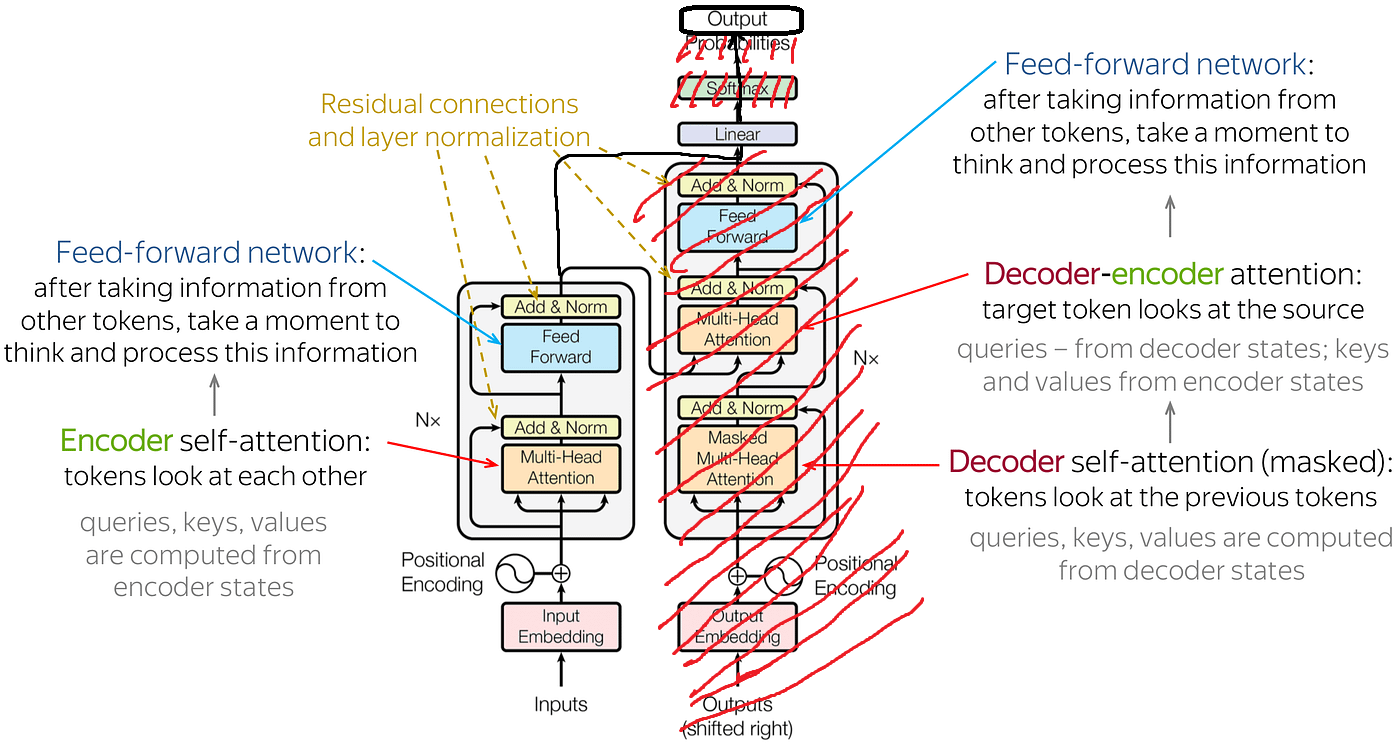
\includegraphics[width=0.5\paperwidth]{images/transformerSeq2Seq.png}
    \caption{A Seq2Seq model from \cite{vaswani2023attentionneed}. The 
    Encoder-only model used in this project, is the same, except the decoder 
    part is skipped, in the image this part has been crossed out with red.}
    \label{fig:transformerSeq2Seq}
\end{figure}

To code this in python an object oriented approach has been taken, with 
classes consisting of other classes, like a matryoshka: 

\begin{itemize}
    \item Multi-Head Attention (MHA) and pointwise-FNN
    \item Encoding layer consisting of the MHA and pointwise-FNN, as well as 
layer normalization and dropout (included in the original paper to prevent 
drop-out)
    \item Encoder containing encoding layers and drop-out.
    \item Transformer which encapsulates embedding and positional encoding, 
as well as obviously the encoder and a final one-neuron-FNN with a linear 
activation.
\end{itemize}

A model with the same hyperparameters like the ones used by \cite{vaswani2023attentionneed} 
can be found in \href{https://github.com/AntonStantan/matura/blob/main/transformer/transformer0.ipynb}
{transformer0}.

Sadly this model get's stuck in a local minimum when training, as you can 
tell at the bottom of it's notebook. The minimum is just predicting a number 
close to 0 for every expression.

We don't want this, so we have to tune the model's hyperparameters.
We do this with the help of keras-tuner. 

A couple of other minor adjustments were made to the model, mainly switching to 
AdamW optimizer, because it is better than Adam for transformers \cite{loshchilov2019decoupledweightdecayregularization}. 
And using a learning rate scheduler with warmup and Cosine decay. This means 
that not like before, when the learning rate stayed constant throughout the 
training, the learningrate changes. It is higher in the beginning and decays 
towards the end. This helps the model take "big steps", "jump over" local 
minimums and take more mindful, careful "steps" towards the end of the training. 

\begin{figure}[htbp]
    \centering
    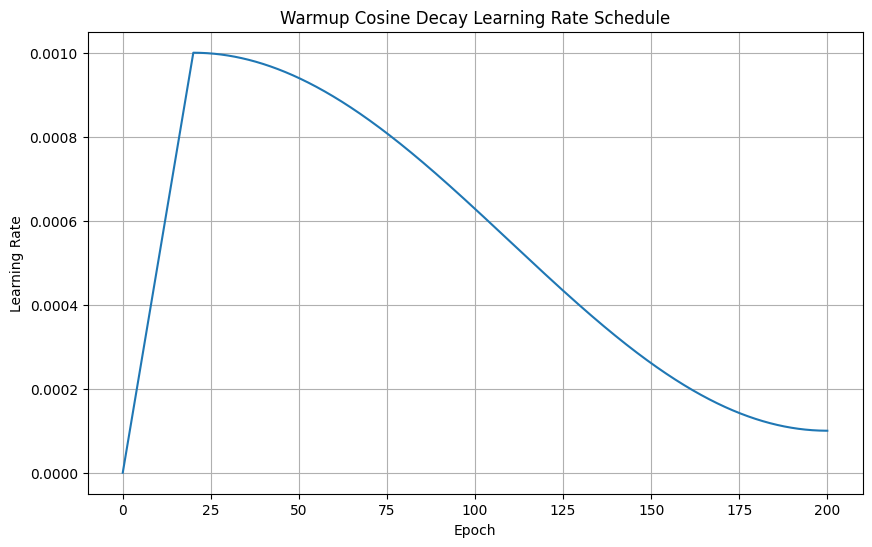
\includegraphics[width=0.5\paperwidth]{images/learningRate.png}
    \caption{This is how the learning rate could look like for a model being 
    trained over the period of 200 epochs, when using a cosine decay with a 
    linear warmup, like in this project. (Except for the changing 
    peak-learningrate all other parameters are the same as the ones used in 
    this project.)}
    \label{fig:learningrate}
\end{figure}

In contrast to the FNN or the RNN a transformer has to be trained on other 
hyperparameters: 
\begin{itemize}
    \item The number of heads inside the MHA
    \item The number of dimensions tensors have inside the model
    \item The number of encoding layers
    \item The number of neurons in the layer inside of the pointwise-FNN
    \item Wether to use dropout or not
    \item The peak learning-rate after warmup and after the cosine decay
\end{itemize}


In the notebooks \href{https://github.com/AntonStantan/matura/blob/main/transformer/transformer4.ipynb}
{transformer4} and \href{https://github.com/AntonStantan/matura/blob/main/transformer/transformer5.ipynb}
{transformer5} you can look at models with successfully tuned 
hyperparameters displaying promising performance on the benchmark.

The difference between them is Transformer5 is a bigger model, than 
Transformer4.

\section{Pre-trained Transformers}

The only model-type left for me to analyse were fine-tuned pre-trained LLMs.
Since working with them is completely different than working with your own 
locally trained neural networks, a lot of research had to be done before 
beginning to dig into the work.
\\[1em]
A lot of fuss went into library compatibility for the amd64 architecture 
system on the Jetson device. The final solution was using a the 
\href{https://github.com/dusty-nv/jetson-containers}{jetson-containers} 
who offer a docker container optimized for the jetson-system. Specifically, 
the container called bitsandbytes has most of the libraries needed for this 
project, the few remaining ones can be installed manually using: \texttt{pip install}


\subsection{Gemini 2.5 Pro}
The first model to be fine-tuned was Gemini 2.5 pro. It is the one I 
personally use the most, it was also chosen in part because of it's high 
ranking in the \href{https://lmarena.ai/leaderboard}{LMarena}. 

Fine-tuning had to be done on a remote server hosted by Google Cloud, 
because of the model's size. 

In the end, the costs for their service amounted to CHF 83.58.

The fine-tuning was done from the VertexAI website. First a .json file with 
the training data had to be created and uploaded. Afterwards the model was 
fine-tuned in the notebook \href{https://github.com/AntonStantan/matura/blob/main/pre-trained-tranformers/gemini_vertex.ipynb}
{gemini\_vertex}. The resulting model is loaded into an endpoint on the 
google cloud servers.

To access the new, fine-tuned model and be able to evaluate it, a pretty 
simplistic notebook is created: \href{https://github.com/AntonStantan/matura/blob/main/pre-trained-tranformers/gemini_vertex_predict.ipynb}
{gemini\_vertex\_predict}

There, the model is loaded in from it's endpoint and used to predict test 
data. 

\subsection{Gemma 3}
For some diversity a smaller (Gemma3 1B parameters) and a tiny (Gemma3 270M 
parameters) were chosen.

Because of their size, they can be fine-tuned locally on the jetson-device.
They are fine-tuned with the SFTTrainer provided by trl.\footnote{We cannot 
use the standard Trainer from huggingface, because the finetuning we do is 
supervised, hence the name: Supervised Fine-Tuning (SFT)} \href{https://huggingface.co/docs/trl/en/sft_trainer}
{The guide on huggingface} was used as help for this.

During the fine-tuning process, a custom designed function that calculates 
the accuracy on some validation data (first 100 samples from the test data). 
This function was used to evaluate the model at different steps in training. 
Fine-tuning notebooks for Gemma3 models can be found under:

\href{https://github.com/AntonStantan/matura/blob/main/pre-trained-tranformers/big_gemma_huggingface.ipynb}{Gemma3 1B}, \href{https://github.com/AntonStantan/matura/blob/main/pre-trained-tranformers/gemma_huggingface.ipynb}{Gemma3 270M}
\\[2em]
After fine-tuning the models can be found in the hugggingface repositories:

\href{https://huggingface.co/AntonBOOM/big_output}{fine-tuned Gemma3 1B}, 
\href{https://huggingface.co/AntonBOOM/output1}{fine-tuned Gemma3 270M}

After a basemodel of the same architecture is loaded with the parameters 
obtained from the fine-tune, see the notebooks: 

\href{https://github.com/AntonStantan/matura/blob/main/pre-trained-tranformers/big_gemma_huggingface_predict.ipynb}{Gemma3 1B prediction notebook}, 
\href{https://github.com/AntonStantan/matura/blob/main/pre-trained-tranformers/gemma-huggingface-predict.ipynb}{Gemma3 270M prediction notebook}

There, the models are used to predict test data and again, calculate the 
accuracy of the respective model.

\subsection{Weird Results Encountered After Evaluation}

A weird observation rose up: The accuracy during the fine-tuning process is 
greater than the accuracy calculated when evaluating the models in the 
prediction notebooks. This is probably due to some error that was overlooked 
but no errors were found.

The error was approached from a systematic standpoint; Multiple hypothesis 
have been set and all of them disproven. The error (if there is one) could 
not be found.

\begin{quote}
\setstretch{0.5}
\footnotesize{
Hypothesis for reason of the error:
	
- There is a previous model that is being loaded, instead of the most recent one. (or not the most recent epoch)

All the previous runs have been deleted, there is only one left. The specific checkpoint has been specified (the most recent one).

- There is an error with generating the data, like using different hyperparameters (temperature and stuff.)

The pytorch .generate() and the huggingface provided generator pipeline both yielded simmilar results. And the pipeline uses hyperparameters from the fine-tune.

- There might be an issue with the calculation during the evaluation steps

I thuroughly checked the compute\_metrics function, and made sure the validation dataset is being used and not the train dataset. The function itself is very basic and there is no error, as confirmed by multiple LLMs.

- The model is overfitted

No, predicting on train data yielded the same (slightly better) results
\\[2em]	
After trying out different checkpoints, all of a sudden the accuracy of the 270m model dropped from 40% to 15%
	
- This lead me to believe maybe it has something to do with the way the models are calculating everything, apart from the temperature and other hyperparameters, it might be because of performance optimization software calculation on GPU or GPU with work offload to CPU might give different results.

Transformers is imported the same way, and is working on GPU exclusively both times.

- Ran the code on the exact same dataset used in the validation part during training. no differences.

- There is a slight difference with the calculation. In the compute metrics function the prediction is only counted if the model uses a turnseparator. This could explain why the seemingly normal gap in accuracies occurred.

After rerunning the training with the correction, the accuracy dropped a little (from 100% to 97%) at the end.

- The pre-trained model obviously has a drop out and layer norms. The issue might be that the model is not in eval mode and is dropping out a lot of valuable data, this would explain the slightly worse performance.

This was not the case, because after setting model.eval() this only increased the accuracy by around half a percent for the Gemma3 270M model, nothing really changed. + This should probably be on by default anyways.

- A perfectly reasonable explanation would be, the model's weights aren't loaded in to the model properly, like it happened with FNN2.ipynb *see 4th of Oct Arbeitsprozess.

This cannot be the case because loading in the hyperparameters is completely different to loading in the weights. A model with loaded-in weights is already trained (hence the name - pre-trained model). Additionally the model is showing signs of having learned from the fine-tuning process for example in the way it responds with the trained Int.0 instead of the traditional Int.
}
\end{quote}
In case you find out why this happens, please contact the author of this 
project.

\newpage
\section{Closing Remark}

The author put a lot of work into this project, he would appreciate all 
sorts of feedback anywhere: from email: anton.mukin@students.ksba.ch, to 
discord: stantan2

Please leave a star on the github repo if you found it interesting.
\\[2em]
I want to thank Herr Schneider for the great insights and quick responses.


\newpage
\printbibliography[heading=bibintoc]

\end{document}
